\chapter{Advertising: Handling Abrupt Phases}

The object of this section is the design a sliding-window combinatorial bandit algorithm for optimizing the budget allocation over the three sub-campaigns in order to maximize the total number of clicks, in the case in which there are the three abrupt phases.
For addressing this assignment \ref{assPart3} we started from the simplified case of one single phase solved in the previous section and we extended it in order to take in consideration the more general scenario of multiple phases.\\

\section{What is an abrupt phase}
Abrupt changes are a specific case of non stationary environment.
In non stationary environments the probability distribution of the random variable associaetd with the reward of every arm can change during time.
Abrupt changes are tipcally associated to new products enter in the market. In this scenario the interests of the cutomers toward the previous towards can decrease abruptly.
In this particular environment the total time horizon is divided in phases and in evey phase the reward function is costant while it changes abruptly between the end of a phase and the beginning of the next one.\\ In Figure \ref{abruptFigure} we can se an example of three different curves generating  the number of clicks, one for each phase, associated to a specific sub-campaign.
\begin{figure}[!htb]
	\centering

	\minipage{0.32\textwidth}
  		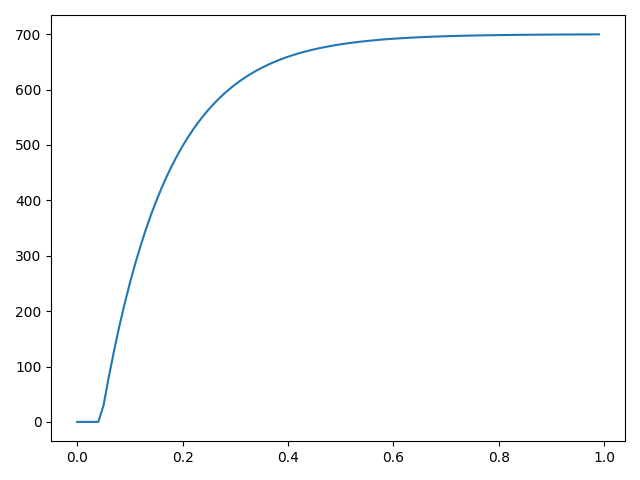
\includegraphics[width=\linewidth]{images/phase0.png}
	\endminipage\hfill
	\minipage{0.32\textwidth}
  		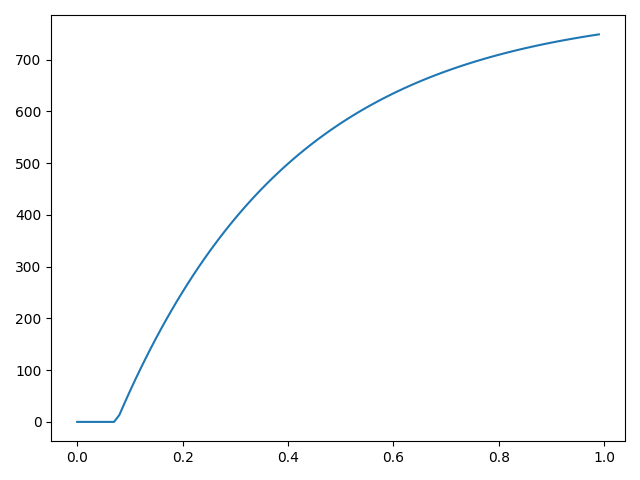
\includegraphics[width=\linewidth]{images/phase1.png}
	\endminipage\hfill
		\minipage{0.32\textwidth}
  		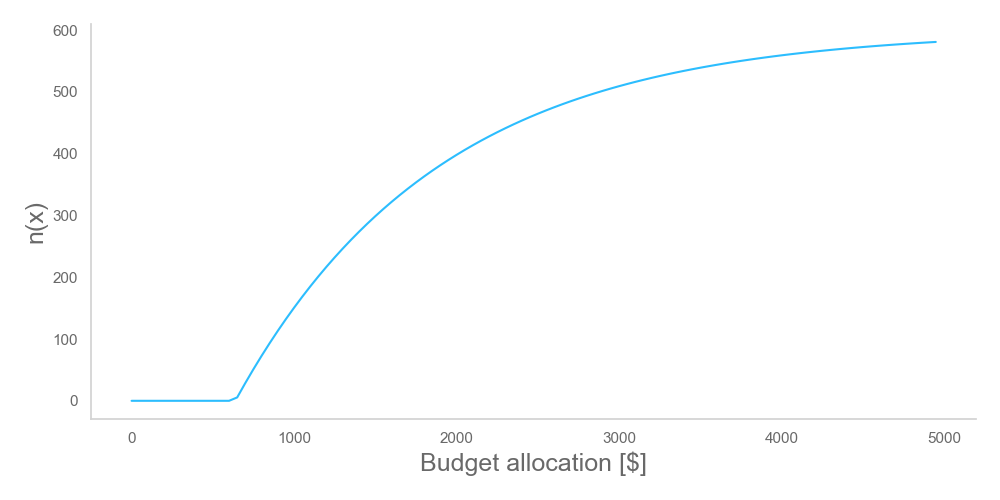
\includegraphics[width=\linewidth]{images/phase2.png}
	\endminipage\hfill
	
	\caption{Example of different curves associated to different abrupt changes}
	\label{abruptFigure}
\end{figure}


\section{Sliding window mechanism}
For this purpose we have implemented the \textit{AbruptBiddingEnvironment.py} class which extends the \textit{BiddingEnvironment.py} class. This class works in a scenario of multiple abrupt phases by returning, for each sub-campaign, the reward of a given pulled arm, depending on the phase we are in.

In this case, the functions generating  the number of clicks given a bid value can change dynamically, according the phase we are in.
The curves differ from the previous definitions only for the dependence to the phase we are in. As follows the mathematical defintion of the three curve functions:

\begin{equation}
	n(x) = c_{M}[phase] \cdot (v_{M}[phase] - e^{-\alpha x})
\end{equation}

We have to remark that the learner is completely transparent with respect to the actually phase we are in and in order to learn the three curves in the case of multiple abrupt phases, we have implemented the \textit{DynamicLerner.py} class as an extension of the standard GP\_Learner.
It implements a \textit{sliding window} mechanism in which we pull a new arm and add the collected rewards until the length of the window is reached. When the window is full, for each new pulled arm we get, we delete the last recent value and add the new one to the collected rewards.\\ Before comparing the performance of this implementation with respect to the one of the standard GP\_Learner, we did a validation in order to understand what is the best length of the window to be adopted. In Figure \ref{winLenValidationFig} the regret associated to three different example of executions of the algorithm with a different windows length. In particular in the plots we can se the regrets in which the length has been set to 33, 67 and 133, i.e. rispectively $\frac{1}{6}$, $\frac{1}{3}$ and $\frac{2}{3}$ of the whole time horizon T = 200 days.
\begin{figure}[!htb]
	\centering

	\minipage{0.48\textwidth}
  		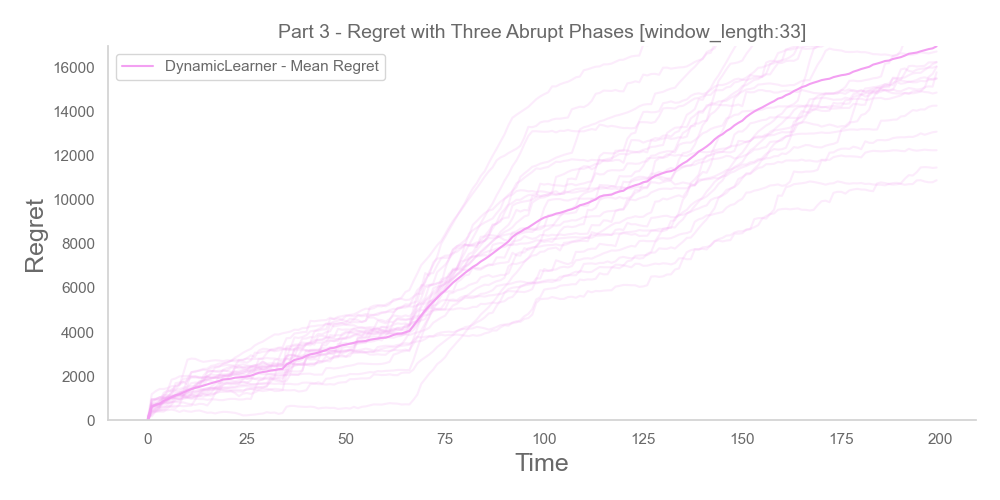
\includegraphics[width=\linewidth]{images/win_length33.png}
  		\caption{Window length = 33}\label{win33}  		
	\endminipage\hfill
	\minipage{0.48\textwidth}
  		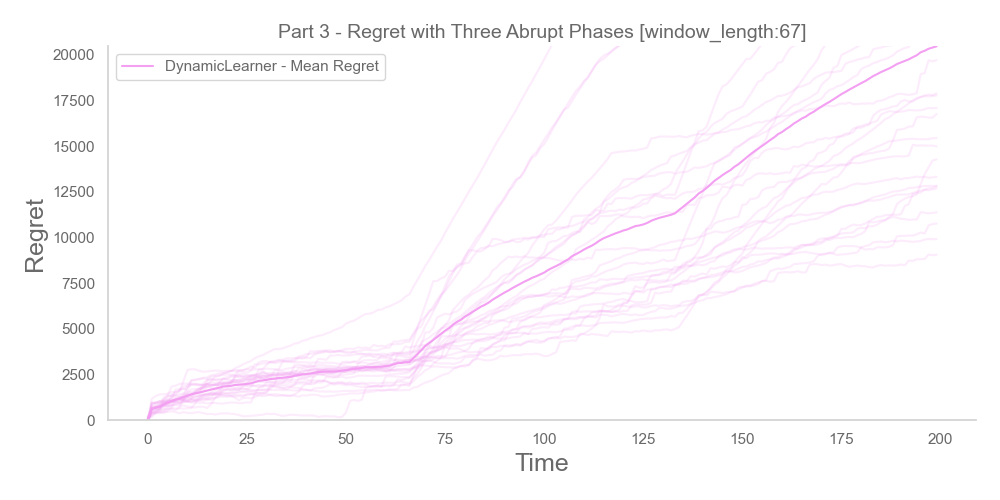
\includegraphics[width=\linewidth]{images/win_length67.png}
  		\caption{Window length = 67}\label{win67}  
	\endminipage\hfill
		\minipage{0.48\textwidth}
  		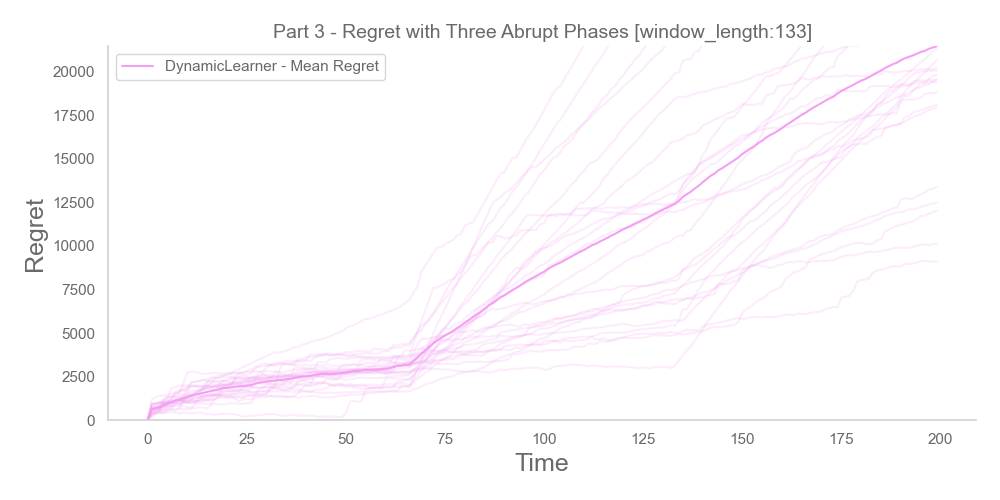
\includegraphics[width=\linewidth]{images/win_length133.png}
  		\caption{Window length = 133}\label{win133}  
	\endminipage\hfill
	
	\caption{\textbf{Tuning in order to find the best window length value}}
	\label{winLenValidationFig}
\end{figure}


As we can notice the performance is highly influenced by the choice of the window length value.
Furthermore all the above results are obtained by running the algorithm over three phases characterized by the same length and so the result can differing more in less specific scenario. For this reason a new method has been designed and implemented to overcome this problem.\\
The final results of the performance of the sliding windows algorithm is for this postponed and it will be analyzed later, in the last section, after the description of the new algorithm we propose.


\section{Changes Detection mechanism}

For solving this problem we have implemented an innovative method which is based on the concept of the \textit{Statistical test}.
We recall that a statistical test is a procedure for deciding whether a hypothesis about a quantitative feature of a population is true or false. Then for testing a hypothesis, we draw a random sample and calculate an appropriate statistic on its items. If, in doing so, we obtain a value of the statistic that would occur rarely when the hypothesis is true, we would have reason to reject the hypothesis.

In our scenario, to detect changes, we need to compare the value of the new drawn sample with the distribution of the points belonging to the same arm in order to decide whether the hypothesis $H_0$,that the new drawn point belongs to that distribution, is true.
Let us suppose to draw a sample whose value is $x_0$ and let $\mu$ $\sigma^2$ be respectively the average
and the standard deviation of the the distribution of the points belonging to the pulled arm. 
If the point doesn't belong to that distribution the hypothesis test should reject $H_0$, with a \textit{confidence interval of 99\%} So we have:

\begin{equation}
	 \mathbb{P}\left(\frac{|x_0 - \mu|}{\sqrt{\sigma^2}} > h \right) = 0.01
\end{equation}

We have that the critical z-score when using a 99\% confidence level are $\pm 2.58$ standard deviations.\\

In the \textit{DLChangeDetect.py} class, we have implemented such change detector. When an arm is pulled more than '\textbf{min\_len}' \footnote{min\_len indicates the minimum number of data we need to have in an arm in order to considere reasonable to run the test} times, for each pull we run the statistical test. When the test reject $H_0$, it means that the point doesn't belong to that distribution and so it means that it is changed. In this case we reset the arm.\\ 
As we did for the sliding window case, also for this algorithm we performed some validation, in order to understand how to properly set the value of the \textit{min\_len}. As follows the plots of the regrets associated to three different example of executions of the algorithm by changing the value of the hyperparameter, i.e. with min\_len equal to 3, 6 and 10 rispectively in Fig \ref{minlen3}, \ref{minlen6}, \ref{minlen10}

\begin{figure}[!htb]
	\centering

	\minipage{0.48\textwidth}
  		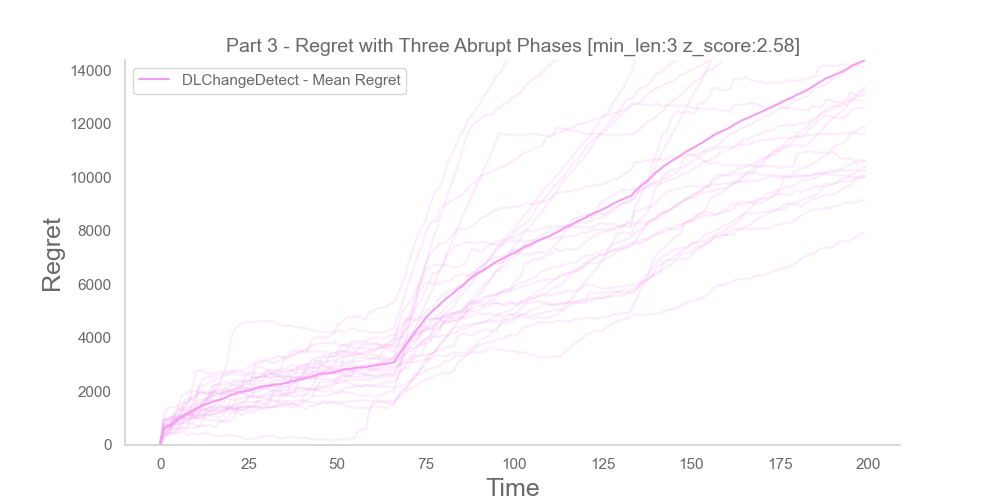
\includegraphics[width=\linewidth]{images/part3_min-len3_z_score2_58.png}
  		\caption{case of min\_len = 3}\label{minlen3}  		
	\endminipage\hfill
	\minipage{0.48\textwidth}
  		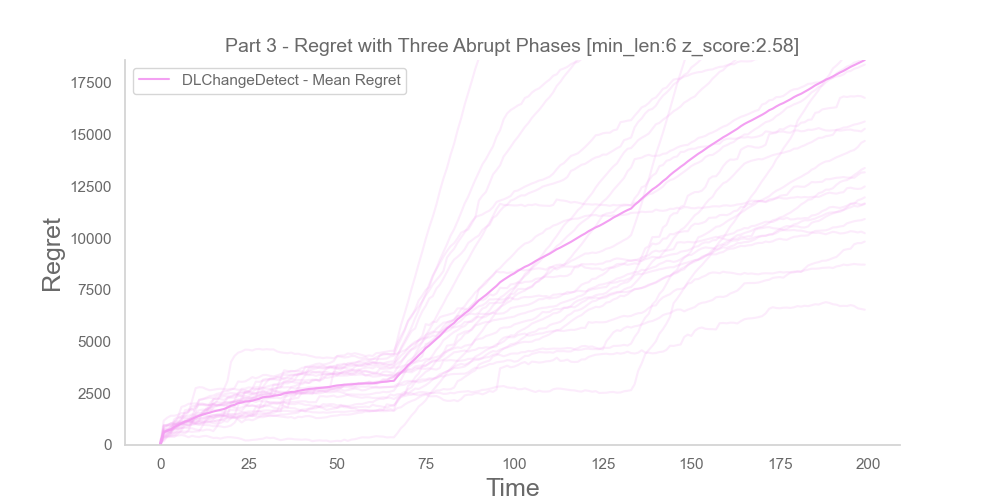
\includegraphics[width=\linewidth]{images/part3_min-len6_z_score2_58.png}
  		\caption{case of min\_len = 6}\label{minlen6}  
	\endminipage\hfill
		\minipage{0.48\textwidth}
  		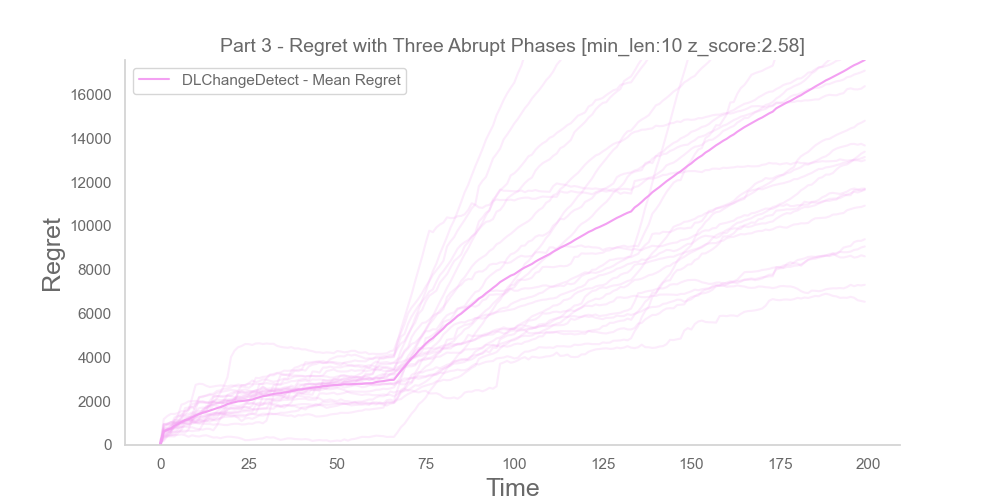
\includegraphics[width=\linewidth]{images/part3_min-len10_z_score2_58.png}
  		\caption{case of min\_len = 10}\label{minlen10}  
	\endminipage\hfill
	
	\caption{\textbf{Selection of the best min\_len hyperparameter}}
	\label{minLenValidationFig}
\end{figure}



Different from before, in this case the performance is not affected from the choice of the min\_len parameter and for this reason, in the final study, we have chosen to run the algorithm by setting min\_len equal to 10, because in this way we consider the arms with more data and so the test can be considered more reliable


\section{Performance evaluation}

This section aims to compare and describe the performance of the three described algorithms.
It is important to remark that in light of the validation we have performed, the comparison are between the standard version of the GP\_Learner, the Dynamic Learnear implementing the sliding window mechanism with window length equal to 33, i.e. on third of the total time horizon of 200 days and the DL\_ChangeDetect learner with min\_len set to 10.
In particular three scenario have been tested:

\begin{enumerate}
\item Three abrupt phases, each phase with a different length
\item Three abrupt phases, all the phases having the same length
\item Four abrupt phases with different length
\end{enumerate}

The first scenario is intended to analyze and compare the performance of the three different algorithms, while the the last two are more specific use cases aimed to compare the behaviour of the Dynamic Learner and the DLChangeDetect learner and to show that the considerations made before actually occur.\\
In Figure \ref{regretPart3CompleteFig} the result of the first scenario is shown. As we can notice, except for the first days in which we have the first phase and so all the learner works similarly, the standard version of the GP\_Learner tends to increase linearly as the number of days increases. On the other hand the two dynamic algorithms both adapts very well to the abrupt changes of the non stationary environment and tend to grows logarithmically. In the plot, we can also see that in this case the DLChange Detector quickly fits the changes while the sliding windows mechanism is slower to learn the changes. Morovere we have that the second phase was very short and this affected drastically the performance of the DynamicLearner and this is consistent to what seen before, because the behaviour of the algorithm depends on the length of the window. 

\begin{figure}[!htb]
	\centering
	%\captionsetup{justification=centering,margin=1cm}
		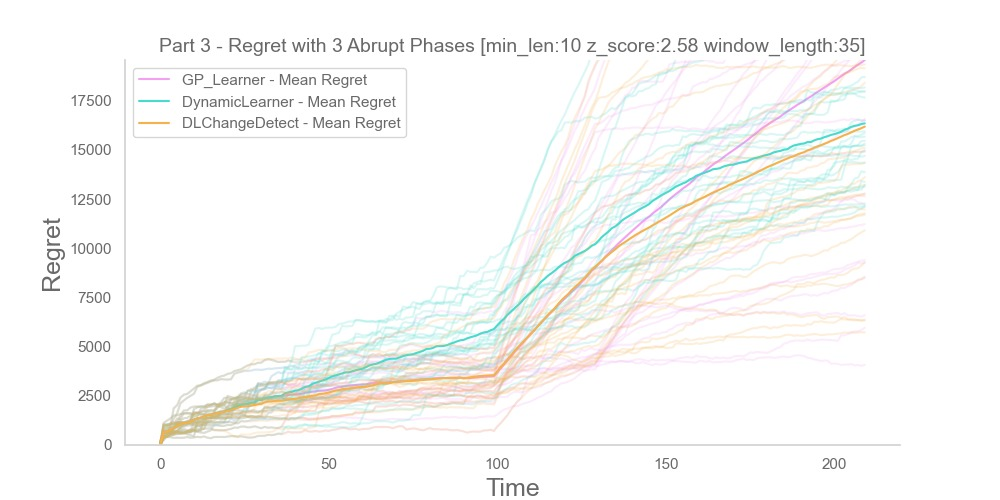
\includegraphics[width=\textwidth]{images/CompleteThreeDifferentPhases.jpeg}
	\caption{Comparison of the three implemented algothims in non stationary environment}.
	\label{regretPart3CompleteFig}
\end{figure}

Finally, as already mentioned, two more specific use cases have been considered. In the following figures we can see the comparison of the regrets of the two implemented algorithms. More precisely in figure \ref{comparisonPlot1} the case of three phases, in which each phases consists of 66 days for a total time horizon of 200 days, while in figure \ref{comparisonPlot2} the scenario of four different phases more precisely of 50, 20, 90 and 40 days.\\ As we can see from the two plots, the DLChange Detector always outperforms the Dynamic Learner.

\begin{figure}[!htb]
	\centering
	%\captionsetup{justification=centering,margin=1cm}
	
	\begin{subfigure}[!H]{0.8\textwidth}
		\centering
		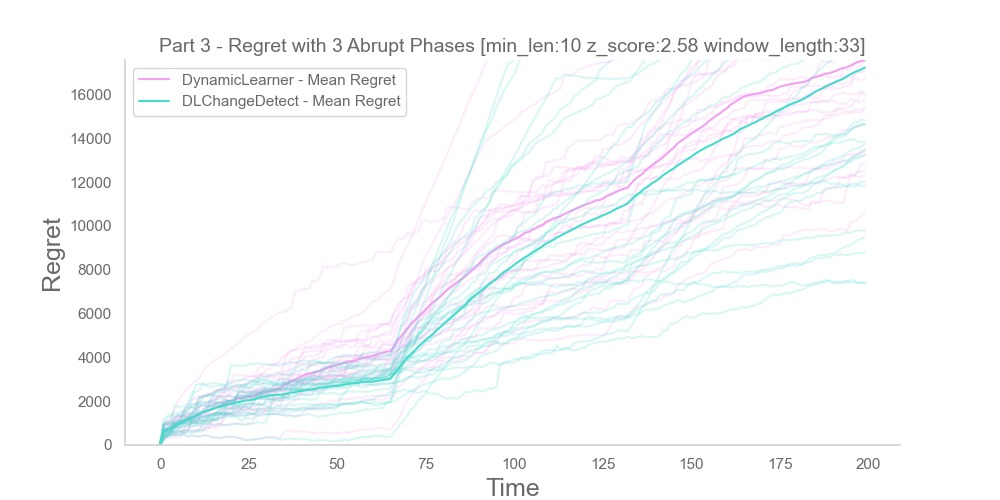
\includegraphics[width=\textwidth]{images/ThreeSamePhase.jpeg}
		\caption{Performance in scenario with three phases with same length}
		\label{comparisonPlot1}
	\end{subfigure}
	%\hfill
	\begin{subfigure}[!H]{0.8\textwidth}
		\centering
		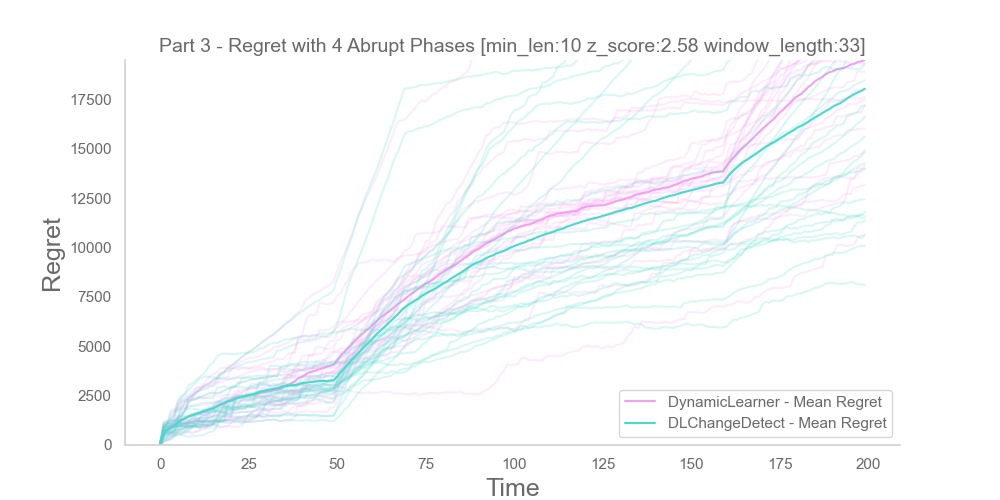
\includegraphics[width=\textwidth]{images/FourAbrupt.jpeg}
		\caption{Performance in scenario with four different phases}
		\label{comparisonPlot2}
	\end{subfigure}
	
	\caption{Comparison between the regrets of the Combinatorial bandit algorithm with a sliding window mechanism and of the Change Detector}
\end{figure}
